%%%%%%%%%%%%%%%%%%%%%%%%%%%%%%%%%%%%%%%%%%%%%%%%%%%%%%%%%%%%%%%%%%%%%%%%%%%

\documentclass{standalone}

\usepackage{amsmath}
\usepackage{mathptmx}
\usepackage{tikz}
\usetikzlibrary{external}
\tikzexternalize{quadratic-as-square}

%% IEEE uses Times Roman font, so we'll default to Times.
%% These three commands make up the entire times.sty package.
\renewcommand{\rmdefault}{ptm}
\renewcommand{\ttdefault}{pcr}
\normalfont\selectfont

%%%%%%%%%%%%%%%%%%%%%%%%%%%%%%%%%%%%%%%%%%%%%%%%%%%%%%%%%%%%%%%%%%%%%%%%%%%
%% A quadratic function interpreted as a square.
%%%%%%%%%%%%%%%%%%%%%%%%%%%%%%%%%%%%%%%%%%%%%%%%%%%%%%%%%%%%%%%%%%%%%%%%%%%

\begin{document}

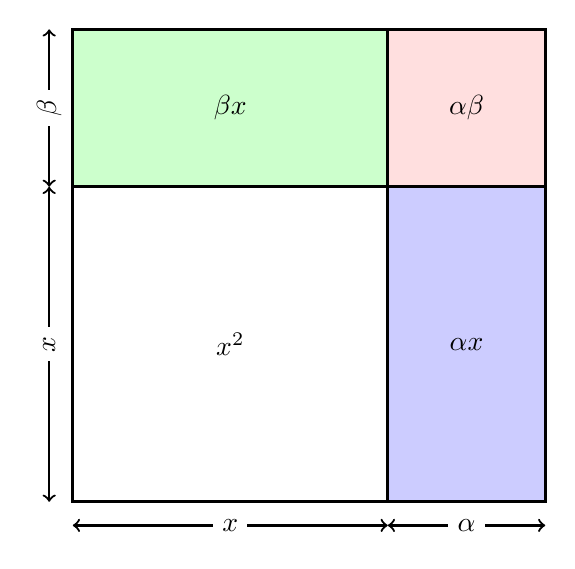
\begin{tikzpicture}[%%
  arrowStyle/.style={<->,thick},%%
  labelStyle/.style={fill=white},%%
  lineStyle/.style={-,very thick}%%
]
%%
%%
\pgfmathsetmacro{\dx}{0.3}
\pgfmathsetmacro{\dy}{\dx}
\pgfmathsetmacro{\length}{4}
\pgfmathsetmacro{\sside}{6}
\pgfmathsetmacro{\width}{2}
\pgfmathsetmacro{\xlow}{0}
\pgfmathsetmacro{\ylow}{\xlow}
%%
%% Larger square.
\coordinate (lowerLeft) at (\xlow,\ylow);
\coordinate (upperRight) at (\sside,\sside);
%%
\normalsize
%%
%% The smaller square.
%% Label the left side of the smaller square.
\draw[arrowStyle] (-\dx,\ylow) -- (-\dx,\length);
\node[labelStyle,rotate=90] at (-\dx,\length/2) {$x$};
%% Label the bottom side of the smaller square.
\draw[arrowStyle] (\xlow,-\dy) -- (\length,-\dy);
\node[labelStyle] at (\length/2,-\dy) {$x$};
%% Label the area of the smaller square.
\node at (\length/2,\length/2) {$x^2$};
%%
%% The top rectangle.
\fill[green!20!white] (\xlow,\length) rectangle (\length,\sside);
%% Label the left width.
\draw[arrowStyle] (-\dx,\length) -- (-\dx,\sside);
\node[labelStyle,rotate=90] at (-\dx,\length+\width/2) {$\beta$};
%% Label the area of the top rectangle.
\node at (\length/2,\length+\width/2) {$\beta x$};
%%
%% The right rectangle.
\fill[blue!20!white] (\length,\ylow) rectangle (\sside,\length);
%% Label the bottom width.
\draw[arrowStyle] (\length,-\dy) -- (\sside,-\dy);
\node[labelStyle] at (\length+\width/2,-\dy) {$\alpha$};
%% Label the area of the right rectangle.
\node at (\length+\width/2,\length/2) {$\alpha x$};
%%
%% The upper-right rectangle.
\fill[pink!50!white] (\length,\length) rectangle (upperRight);
\node at (\length+\width/2,\length+\width/2) {$\alpha\beta$};
%%
%% The larger square.
\draw[lineStyle] (lowerLeft) rectangle (upperRight);
%% Divide the larger square into rectangles.
\draw[lineStyle] (\xlow,\length) -- (\sside,\length);
\draw[lineStyle] (\length,\ylow) -- (\length,\sside);
\end{tikzpicture}

\end{document}
